\chapter{Motor control}

\subsection*{ Angular velocity control}

In previous work, two controllers a linear and a non-linear(SMC), have been designed requiring a torque that has to be produced from the motors-wheel system. This torque demand is used to give the desired angular velocity reference for the wheels and thus the torque that will be fed back to the satellite as seen in the \cite{block diagram}. The output torque from the linear and non-linear controllers has three elements which has to be transformed in the tetrahedron configuration using the matrix \eqref{transmatrix}.  A \textit{PID} controller has been designed to control the angular velocity of the motor as seen in the \figref{fig:blockdi222}:
\begin{figure}[H]
	\centering
	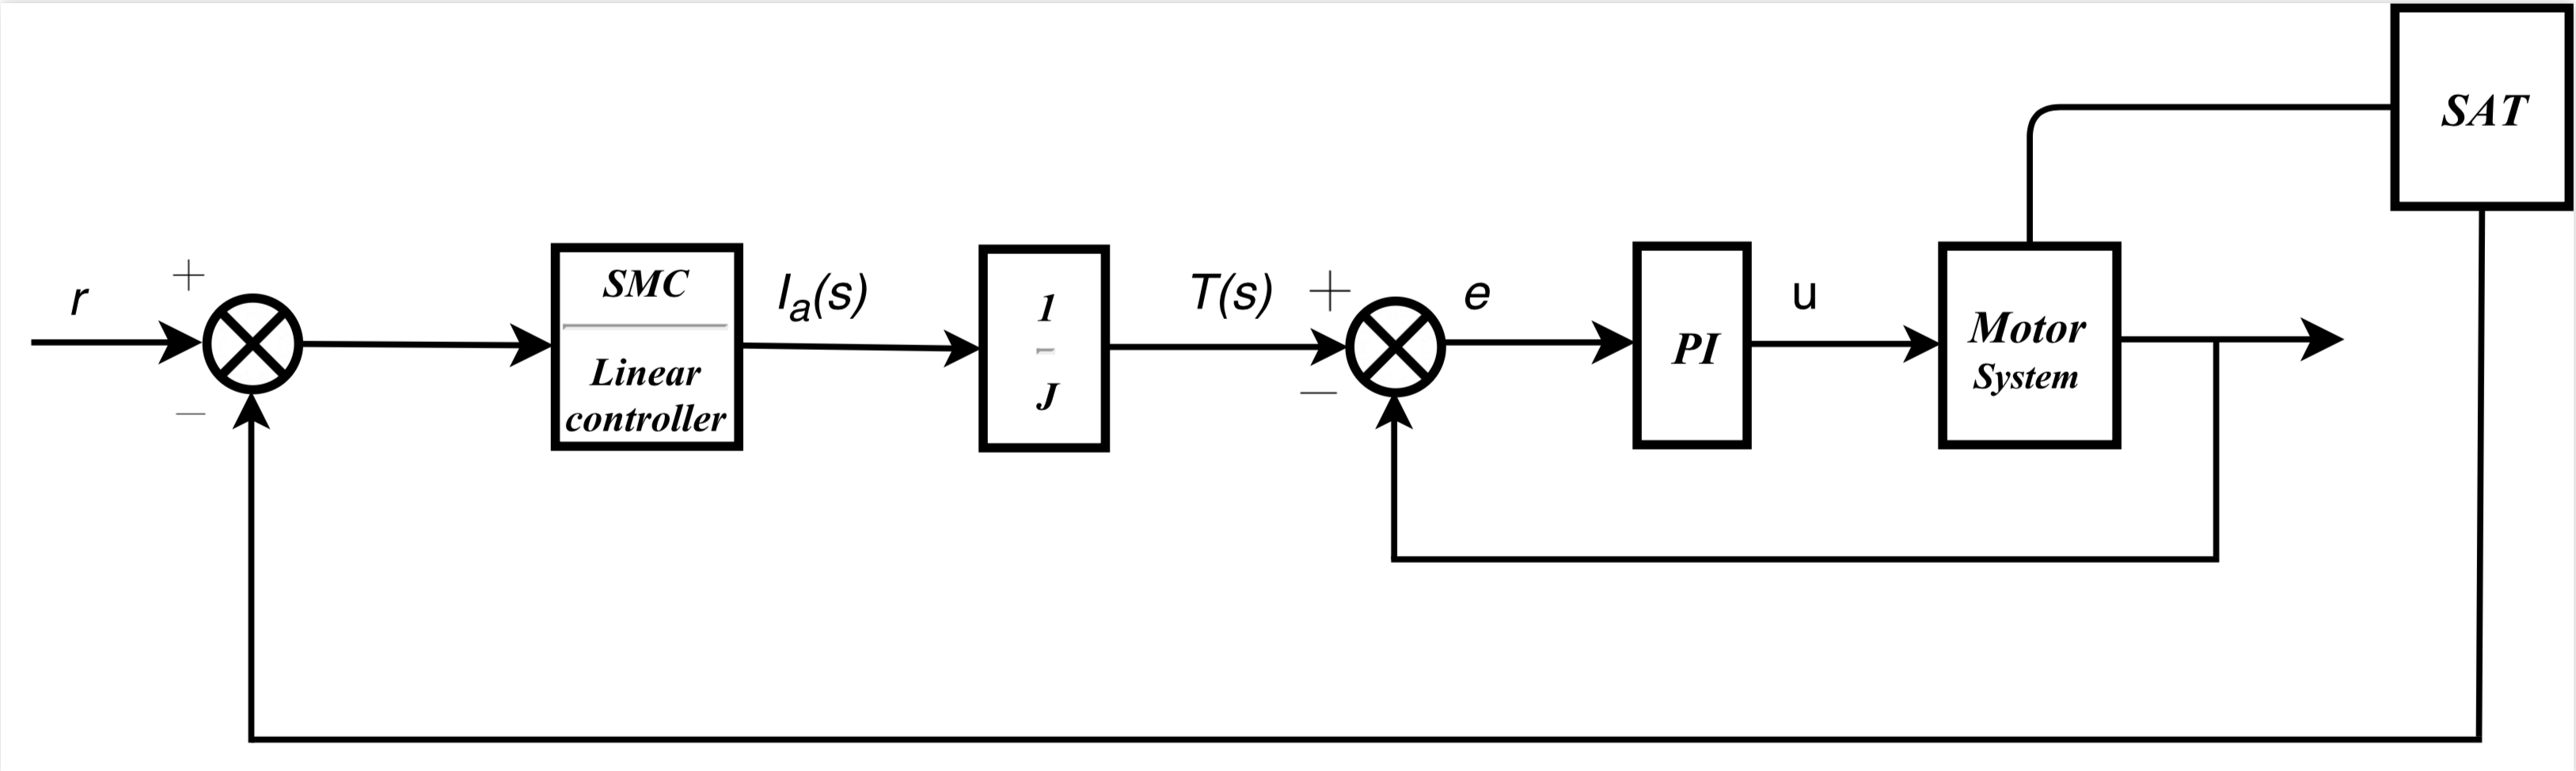
\includegraphics[width=1.0\linewidth]{figures/block_diagram_2}
	\caption{Block diagram of the motor control with PID controller}
	\label{fig:blockdi222}
\end{figure}  
%
The PI controller gains are chosen based on the open loop system response using the Ziegler-Nichols method \cite{PID_tuning} and by trial and error in order to achieve faster closed loop response and asymptotically stable system. The gains are chosen to be:   
%
\begin{flalign*}
	k_{p} = 3.4 \\ k_{i} = 0.9
\end{flalign*}